\documentclass[a4paper,11pt]{scrartcl}
\usepackage[french]{babel}
\usepackage[utf8]{inputenc}
\usepackage[T1]{fontenc}
\usepackage{pst-all}
\usepackage{vanadin}
\usepackage{isotope}
\usepackage{longtable}
\usepackage{color}


\subject{TP~3 Physique nucléaire}
\title{Perte d'énergie des particules $\alpha$ dans l'air}
\subtitle{Particules $\alpha$ dans l'air}
\author{Mona Dentler, Sabine Engelhardt}
\publishers{Université Joseph Fourier, Grenoble}
\date{\today}

\begin{document}
 \pagestyle{empty}
 \begin{center}
  \makeatletter
   %\titlefont
  \@subject
  \vspace{2cm}

  \Huge
  Perte d'énergie des particules $\alpha$ dans l'air\newline
  \vspace{1cm}
  \Large


  \@author
  \newline
  \@publishers


  \@date
  \makeatother
 \end{center}
 \vfill

 \textcolor{blue}{Sabine}
 \textcolor{red}{Mona}

 \begin{abstract}
  Le but des cette TP est de connaître la perte d'énergie des particules $\alpha$ dans l'air. Nous avons eu deux sources une source d'Americium 241 (\isotope[241]{Am}) et une source de Plomb 212/ Bismuth 212 (\isotope[212]{Bi}) pour étudier des particules $\alpha$ différentes. L'$\alpha$ perd son énergie par ionisation des atomes de la matière, ici l'air. La perte est proportionnelle au carré de la charge et à la masse de l'$alpha$ et varie beaucoup avec la vitess d'$\alpha$. Plus l'$\alpha$ est lente plus de temps il passe dans l'atome et \c ca augmente la chance d'une interaction. Si l'ionisation est très intense, le trajet de la particule est très court.

  Dans ce TP nous allons étudier le spectre des $\alpha$ émis par les deux sources, calibrer le dispositif éxpermental pour ensuite mesurer le pouvoir d'ionisation des $\alpha$. C'est réalisé par la mesure de la longuer du trajet des $\alpha$ dans l'air.
 \end{abstract}
\newpage
 \pagestyle{scrheadings}
 \tableofcontents
\newpage

 \begin{section}{Etude des sources}
  \begin{subsection}{La source \isotope[241][95]{Am}}
   La période de l'\isotope[241][95]{Am} est \unit[432,6]{ans} et ce noyeau se désintègre vers le \isotope[237][93]{Np}. A presque \unit[100]{\%} des désintégration sont des désintégration $\alpha$, seule $\unit[4,3\cdot10^{-10}]{\%}$ 
   se fait par fission spontanée.  

   \todo{Schema malen}

   Le énergie cinétique d'un $\alpha$ est équivalent à la diffénce d'énergie causé par le défaut de masse entre les particules. Alors l'énergie cinétique de trois $alpha$ principaux se calculent comme suivante:
   \begin{equation*}
    T=\Delta E\stackrel{Einstein}{=}\Delta M\cdot c^2=\left(M\left(\isotope[241]{Am}\right)-M\left(\isotope[237]{Np}\right)-M\left(\isotope[4]{He}\right)\right)c^2\approx\unit[5,638]{MeV}
   \end{equation*}
   avec $M\left(\isotope[241]{Am}\right)=\unit[241,0568229]{uma},M\left(\isotope[237]{Np}\right)=\unit[237,0481673]{uma}, M\left(\isotope[4]{He}\right)=\unit[4,00266032]{uma}\text{ et }\unit[1]{uma}\cdot c^2=\unit[931,5]{MeV}$.

   Les trois $\alpha$ principaux sont ceux avec la plus grande possibilité d'être émis, ici ce sont les $\alpha$ émis par la désintegration vers \isotope[237]{Np^*} $\nicefrac{5}{2}^-$ avec \unit[84,85]{\%}, la désintegration vers \isotope[237]{Np^*} $\nicefrac{7}{2}^-$ avec \unit[13,23]{\%} et la désintegration vers \isotope[237]{Np^*} $\nicefrac{9}{2}^-$ avec \unit[1,66]{\%}.
   \begin{eqnarray*}
    T_{\nicefrac{5}{2}^-}=T-E^*_{\nicefrac{5}{2}^-}=\unit[5,578]{MeV}\\
    T_{\nicefrac{7}{2}^-}=T-E^*_{\nicefrac{7}{2}^-}=\unit[5,535]{MeV}\\
    T_{\nicefrac{9}{2}^-}=T-E^*_{\nicefrac{7}{2}^-}=\unit[5,479]{MeV}
   \end{eqnarray*}
  \end{subsection}
 
  \begin{subsection}{La source \isotope[212][83]{Bi}}
   Le \isotope[212][83]{Bi} fait partie de la chaîne radioactive du Thorium 232. Car le  \isotope[212]{Bi} n'a qu'une période de \unit[60,5]{min}, la source a été apporté par un technicien pendant la TP. Le [212]{Bi} se désintègre vers le Thalium \isotope[208][81]{Tl} en émettant des particules $\alpha$ \isotope[4][2]{He} et vers le Polonium\isotope[212][84]{Po} par désintégration $\beta^-$ comme le schéma suivant le montre.

   \todo{Schema Bismuth}

   Le Polonium \isotope[212][84]{Po} fait à son tour par \unit[100]{\%} la désintégration $\alpha$ vers le plomb \isotope[208][82]{Pb} avec une période de $T=\unit[298]{ns}$.

   \todo{Schema Pollonium}

   Les trois $\alpha$ principaux sont deux $\alpha$ de la désintégration vers le \isotope[208]{Tl} et l'$\alpha$ de la désintégration du \isotope[212]{Po} avec les énergies suivantes. Pour 100 désintégration du \isotope[212]{Bi} environ 90 particules $\alpha$ sont émis.
   \begin{eqnarray*}
    T_1=\left(M\left(\isotope[212]{Bi}\right)-M\left(\isotope[208]{Pb}\right)-M\left(\isotope[4]{He}\right)\right)c^2\approx\unit[6,154]{MeV}&\text{ avec }\unit[9,7]{\%}\\
    T_2=T_1-E^*_{4^+}=\unit[6,114]{MeV} &\text{ avec }\unit[25,1]{\%}\\
    T_3=\left(M\left(\isotope[212]{Po}\right)-M\left(\isotope[208]{Pb}\right)-M\left(\isotope[4]{He}\right)\right)c^2\approx\unit[8,901]{MeV} &\text{ avec }\unit[55,2]{\%}    
   \end{eqnarray*}
   avec $M\left(\isotope[212]{Bi}\right)=\unit[211,9912715]{uma},M\left(\isotope[208]{Tl}\right)=\unit[207,9820047]{uma}, M\left(\isotope[212]{Po}\right)=\unit[211,9888518]{uma},\newline M\left(\isotope[208]{Pb}\right)=\unit[207,9766359]{uma}, M\left(\isotope[4]{He}\right)=\unit[4,00266032]{uma}\text{ et }\unit[1]{uma}\cdot c^2=\unit[931,5]{MeV}$.
   
   On peut se poser la question pourquoi la désintégration du \isotope[212]{Bi} vers l'état fondamental est plus probable que vers le deuxième état excité parce qu'ils ont tous les deux le même moment angulaire et la même parité $5^+$. C'est assez facile à comprendre car les atomes vont avoir un état énergétiquement favorable, c'est à dire un état stable. Comme l'état fondamental est le plus stable des deux états la désintégration vers l'état fondamental est préféré.

   Le \isotope[212]{Po} a une période très court à cause de la préférence d'un noyeau avec un nombre magique. Le \isotope[208][82]{Pb} est un noyeau double magique avec le nombre magique 84 pour les protons et le nombre magique 126 pour les neutrons. Alors ce noyeau est fortement favorisé du noyeau de \isotope[212]{Po}.
  \end{subsection}
 \end{section}

 \begin{section}{Dispositif expérimental}
   Le dispositif expérimental se compose d'un enceinte à vide et ses accesoires, un détecteur rélie à un préimplificateur et un analyseur multicanal. Le siganl est enregisté sur l'ordinateur par un logiciel très simple.
   
   \begin{subsection}{Enceinte à vide}
    Dans l'einceinte à vide se trouve le détecteur et un sélecteur de source pour que nous n'ayons pas dû toucher les sources nues $\alpha$ se qui est très dangereux et peut causé de cancer. En plus il y a une pompe pour faire le vide et un système de vanne et de fuit micrométrique pour faire rentrer l'air précisement. Un jauge capacitif calibré parun jauge Pirani très précis mesure la pression dans l'enceinte avec une précision de \unit[0,2]{\%}.  
   \end{subsection}

   \begin{subsection}{Détecteur et préamplificateur}
    \begin{figure*}[hbt]
     \begin{center}
      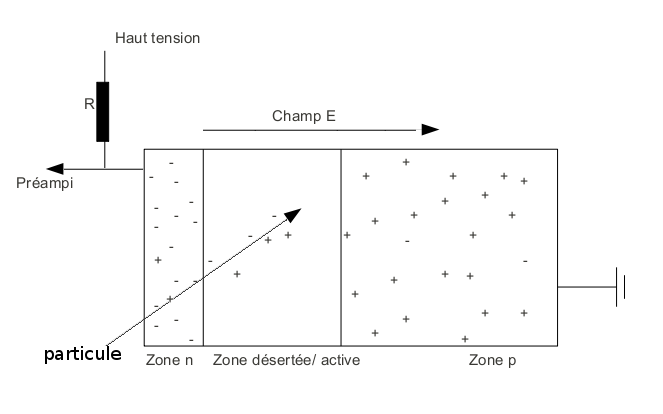
\includegraphics[width=0.75\textwidth]{Bilder/detecteur.png}
     \end{center}
     \caption{schéma d'un détecteur semi-conducteur}
    \end{figure*}
    Le détecteur est un détecteur semi-conducteur et consiste d'une jonction Si(Li) avec une barrière de surface. Un détecteur semi-conducteur a trois parts: une zone chargée négative n, une zone chargée positive p  et une zone neutre, la zone active ou desertée. Le largeur de cette dernière zone est reglée par haute tension, la tension de polarisation. Comme ci la jonction est assimilable à un condensateur plan dont la distance est égale à la zone désertée. Donc ce condensateur est de même d'amplitude que la tension rélié.

    Le préamplificateur de charge supprime ce problème. Il est rélie à un module de mise en forme qui fournit un signal de l'amplitude proportionnel à la charge collecté dans la jonction du détecteur indépedant de la capacité.
   \end{subsection}

   \begin{subsection}{Logiciel}
    Un amplificateur entre le préamplificateur et l'analyseur d'amplitude donne la possibilité d'ajuster le signal à un valeur connue. L'analyseur d'amplitude est rélie à l'ordinateur où un logiciel montre le signal en fonction de l'énergie d'$\alpha$. Ce logiciel n'est pas calibré alors il faut le faire soi-même et il permet de choisir la temps de la mesure et un seuil qui était mis à \unit[200]{mV}.
   \end{subsection}
  \end{section}
  
  \begin{section}{Expériences préliminaire}
   \begin{subsection}{Etude de la réponse du détecteur}
    \begin{subsubsection}{Caractéristique du détecteur}
    \todo{Astar}
    \end{subsubsection}
    \begin{subsubsection}{Largeur de la zone active en fonction de la tension}
     Pour comprendre le comportement du détecteur en fonction de la tension, nous avons lancé une série de mesure. Nous avons choisi une tension de \unit[0]{V}, \unit[25]{V}, \unit[50]{V} et \unit[80]{V}.
     \todo{résultats, Erklärung und was haben wir weiter genutzt}
    \end{subsubsection}
  \end{subsection} 

  \begin{subsection}{Calibration des résultat}
    
  \end{subsection}
  
  \begin{subsection}{Simulation de la perte d'énergie}
   
  \end{subsection}
 \end{section}

 \begin{section}{Mesure}
  
 \end{section}

 \begin{section}{Conclusion}
  Nous avons appris comment lancé une mesure et calibré les dispositifs pour cette mésure. En plus nous avons vu que des particules $\alpha$ déposent leur énergie après un certain trajet parcouru. Cette distance montré par le pic de Bragg est spécifique pour les $\alpha$ d'une source comme nous avons vu en comparaisant les deux sources disponibles pour la TP.
  
  Dans la radiothérapie on use ce fait pour détruire des tumeurs. En utilisant des particules $\alpha$ on est sûre de ne détruire que la tumeur car l'alpha interagissent que dans cette pétite zone bien défini.
 \end{section}

 \vspace{1cm}
 \begin{flushright}
  \titlefont \textcopyleft\ Mona Dentler et Sabine Engelhardt
 \end{flushright}

\end{document}

